% Created 2021-06-14 Mon 18:59
% Intended LaTeX compiler: pdflatex
\documentclass{article}
\usepackage[utf8]{inputenc}
\usepackage[T1]{fontenc}
\usepackage{graphicx}
\usepackage{grffile}
\usepackage{longtable}
\usepackage{wrapfig}
\usepackage{rotating}
\usepackage[normalem]{ulem}
\usepackage{amsmath}
\usepackage{textcomp}
\usepackage{amssymb}
\usepackage{capt-of}
\usepackage{hyperref}
\usepackage[margin=2cm]{geometry}
\usepackage[a4paper,bindingoffset=0.2in,left=1in,right=1in,top=1in,bottom=1in,footskip=.25in]{geometry}
\usepackage[backend=biber,style=apa]{biblatex}\addbibresource{/Users/ricmagno/Documents/References/library.bib}
\addbibresource{/Users/ricmagno/Documents/References/library.bib}
\usepackage{tikz}
\author{Ricardo Antunes, Vicente A. González, Kenneth Walsh, Michael O'Sullivan, and Omar Rojas}
\date{\today}
\title{Productivity Function\\\medskip
\large Mathematical foundation for Production Management in Construction}
\hypersetup{
 pdfauthor={Ricardo Antunes, Vicente A. González, Kenneth Walsh, Michael O'Sullivan, and Omar Rojas},
 pdftitle={Productivity Function},
 pdfkeywords={},
 pdfsubject={Chapter Proposal},
 pdfcreator={Emacs 26.3 (Org mode 9.1.9)}, 
 pdflang={English}}
\begin{document}

\maketitle
\tableofcontents

1;95;0c:PROPERTIES:
:ID:       170029D7-DE41-4BDB-B78E-54BCEA47E375
:END:


\section{Guidelines}
\label{sec:org29aeb15}
\begin{verbatim}
'(tex-count-word)
\end{verbatim}

\begin{itemize}
\item 7000 Words
\end{itemize}

\section{Abstract}
\label{sec:org07820cb}
The building construction industry faces challenges, such as increasing project complexity, and larger scope requirements but shorter deadlines. 
Additionally, the industry relies on practices based on intuition and experience, overlooking the dynamics of its production system. 
These approaches underestimate the influence of process repetitiveness, the size of the production run, the transient state (setup times), the variation of learning curves, and the conservation of processes properties. 
Consequently, construction adopts the manufacturing production model dismissing the application of approaches that accurately describe the characteristics of its production system. 
This chapter aims to provide a production theory to better understand the production mechanisms of repetitive processes in project-driven systems in construction.
The chapter begins with an examination of the existing knowledge about production models, their characteristics, and the challenges to establishing a theoretical framework for controlling dynamic production systems management in construction projects. 
The chapter progresses to an analytical and scalable method (Productivity Function) to represent the behavior of production systems. 
The Productivity Function provides a mathematical foundation for the calculations of cycle times (average, best- and worst-cases), throughput at capacity, and the influence of the transient state time in the production variability. 
Productivity Function is applied in feedback loop control yielding a robust approach to plan, control, and optimize production.
Finally, the chapter presents automated methods of data collection that feed the Productivity Function models, which are the foundation of the production theory and support the decision-making process on Lean Construction 4.0. 

\section{Introduction}
\label{sec:orgb7b9d41}
Despite the name of the title of this chapter, you will not find equations here.
Not because they do not exist, but because we believe that, at least for now, it is more important to understand what these equations represent than how they come to be.
You are welcome to deep your knownledge and see the equations and their development on the referenced literature.
\section{Lean principles and production theory [0/2]}
\label{sec:orge922e69}
\subsection{Production in manufacturing (Factory Physics)}
\label{sec:orga66a3b6}
The manufacturing industry is knowable of its production.
From early times when 'time and motion' has been developed on workers construction a brick wall (Reference here), manufacturing has being advancing on undestanding and manageming of its production.
Mostly important on the context on this book, it was the creation and development of lean production that inspired lean construction.
This chapter stands on further development of lean production: it's mathematical explanation of production.
Such work has been conducted by TOYOTA dude, THE guy from MIT and mates from Factory Physics.
Their work combined provide a set of equations that apply to manufacturing production systems.
A production system consists into three main elements: inputs, process, outputs (Figure ).
Inputs may not reflecet the full range of requirementes to create the output but on this system view they determine the output.
The process can be determined on physical knwon equations or most oftern determined by evaluating the relationship betwen input and output.
The mathematical representation of this relantionship is main difference between manufacturing and construction.

\subsubsection{Throughput \label{throughput}}
\label{sec:orgb8be5f4}

Throughput, TH, is the number of production units sold per unit of time \citep{Hopp2001}.
However, throughput in production systems, THs, has a slightly different meaning.
THs is the number of units produced per unit of time or the production system throughput rate.
Throughput is the output frequency.
The value of TH is presented as the average value of the production system throughput rate.
THs does not generate revenue; it creates an inventory.
THs is utilized to measure the performance of an individual production process and or routings in a network of transformations processes.

\subsubsection{Capacity \label{capacity}}
\label{sec:orgfe7bf62}

Capacity is the maximum number of units that a production system releases per unit of time \citep{Hopp2001}.
Capacity is equivalent to the maximum throughput.
Maintaining a production system at capacity is complex.
Because most production systems are unstable at capacity, releasing work at unsteady rates.
That disturbs the flow and process THs, consequently producing irregular intermediate inventories between these processes.

\subsubsection{Work-in-process}
\label{sec:orgcc775eb}

Work-in-process, WIP, consists of the intermediate inventories between transformation processes.
WIP excludes the inventories at the extremes of the production chain, i.e., the first raw material inventory and the finished goods inventory \citep{Hopp2001}.

\subsubsection{Cycle time \label{cycle_time}}
\label{sec:orgff812de}

The cycle time, CT, is the time spent to produce a good, i.e., complete a production cycle.
Cycle time measures the time a product or a service takes to be completed \citep{Hopp2001}.
Alternatively, CT is also utilized to measure the performance of an individual transformation process or routing in a network of transformations processes.

In production, the \(\mbox{CT}_1\) is the time taken to manufacture the first product.
It is also know at Lead time (\ref{lead_time}).
However, \(\mbox{CT}_2\) is the time between the release of the first product and the second.
\(\mbox{CT}_2\) should be considerably smaller than \(\mbox{CT}_1\) because at the time the first product is released, the next product should be queued at the last transformation product.
Consequently, the time necessary for releasing the next product is equivalent to the processing time to finish the next product.
In this case, \(\mbox{CT}_2\) is equal the CT of the last transformation process.

\subsubsection{Lead time \label{lead_time}}
\label{sec:org9d83f51}

Lead time, LT, is the time assigned for production between the start and end of the transformation process chain \citep{Hopp2001}.
The start and end of lead time are at the same points those in of cycle time.
The difference is that lead time is allotted and cycle time is measured.
Lead time is a management constant.
During normal operations, the cycle time is less or equal than the lead time.

\subsubsection{Utilization \label{utilization}}
\label{sec:orgc856682}

Utilization is the ratio of the actual output to the full potential output of a transformation process expressed as a percentage.
The actual output and the full potential may be expressed in currency units, unit amount of production or time, whichever provides better management information \citep{Kumar2009}.
The difference between actual and potential output (measured by the utilization ratio) can be used to display potential problems in the process, such as machine failure, job waiting, or lack of parts.
As mentioned above, a few processes operate at capacity due to stability issues.
As a result, utilization is also rarely close to 100\%.
If utilization is high, the process is operating under capacity.
Conversely, low utilizations indicate an excess of capacity \citep{Hopp2001}.

\subsubsection{Law (Little's Law) \label{littles_law}}
\label{sec:org2d90297}

Named after John D. C. Little \citep{Little1961}, the Little's law relates three of main lower level variables management in a queuing system.
A queuing system consists of a flow of discrete items arriving at a constant pace, to a stable system that services and releases these items for further processing.
The system follows a First-In, First-Out (FIFO) sequencing.
Figure\textasciitilde{}\ref{fig:Schematic view of a flow of items through a queuing system} shows a schematic view of a flow of items through a queuing system.

\begin{figure}[H]
  \centering
  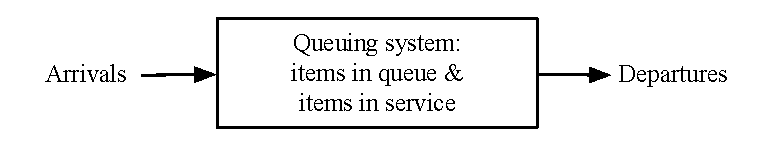
\includegraphics[width=1\linewidth]{Figures/LiteratureReview/Schematic_view_of_a_flow_of_items_through_a_queuing_system}
  \caption{Schematic view of a flow of items through a queuing system}\label{fig:Schematic view of a flow of items through a queuing system}
  \source{Adapted from citep:Little2008}
\end{figure}

Little's Law states that, under steady state conditions, the average number of items in a queuing system equals the average rate at which items arrive multiplied by the average time that an item spends in the system \citep{Little2008}.

Furthermore, there is not a unique solution for the formula because there are no constants involved.
It is possible to obtain a value of \(L\) with infinite combinations of \(\lambda\) and \(W\).
Another important remark about Little's law is the assumption of a stationary arrival process.
A more precise realization of a particular queuing system is possible for Little's Law by interpreting the number of items arriving and departing in the system, as shown in Figure\textasciitilde{}\ref{fig:Number of items in a queuing system versus time}, where:

To obtain \(L=\lambda \times W(T)\), the system must be at steady state, i.e., \(T \rightarrow \infty\).
Therefore:

\begin{figure}[H]
  \centering
  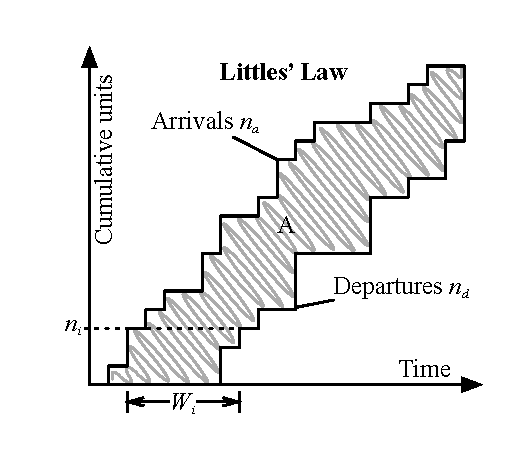
\includegraphics{Figures/LiteratureReview/Number_of_items_in_a_queuing_system_versus_time}
  \caption{Number of items in a queuing system versus time}\label{fig:Number of items in a queuing system versus time}
  \source{Adapted from citep:Little1961}
\end{figure}

Over the years, the original Little's law equation \citep{Little1961} evolved to a more generic form comprising operations management \citep{Hopp2001}.
Work-in-process, WIP, is equivalent to the expected number of units in the system, \(L\).
The average output of a production process per unit time, THs, is the arrival rate during period, \(\lambda\), and the cycle time, CT, is the average waiting time in the system per arrival during \(T\), \(W\).
Thus, Little's Law can also be written as:

\begin{equation}
  \mbox{WIP} = \mbox{CT} \times \mbox{TH}
   \label{eq:Little's Law for operation management}
\end{equation}

The difference between Equation\textasciitilde{}\ref{eq:Little's Law} and Equation\textasciitilde{}\ref{eq:Little's Law for operation management} is crucial in this research because project-driven production is seldom at steady state.
Consequently, the Equation\textasciitilde{}\ref{eq:Little's Law for operation management}, which is based on an average behavior of variables over a very long period, is likely to produce an imprecise approximation.
However, to describe most relations of production in manufacturing the approximation described in Equation\textasciitilde{}\ref{eq:Little's Law for operation management} is sufficiently accurate.


\subsubsection{Bottleneck rate}
\label{sec:org6c23093}
In a production line, the bottleneck rate, \(r_b\), of this line is given by the throughput of the process with highest long-term utilization, i.e., lowest effective rate \citep{Hopp2001}.
In general terms, the bottleneck rate points out the process that is working closest to its capacity.
Accordingly, the bottleneck process restricts the throughput of the production line.

\subsubsection{Critical WIP}
\label{sec:orgddf9039}

The critical WIP, \(W_0\), of a production line, is the value related to the maximum production capability \citep{Hopp2001}.
At \(W_0\) the production line reaches its maximum throughput, \(\mbox{THs}_{\mbox{max}}\), restricted by \(r_b\), producing goods with minimum intervals, i.e., cycle time \(\mbox{CT}_0\) \citep{Martin1998}.
Hence, according to Little's law, the critical WIP is given by Equation\textasciitilde{}\ref{eq:Critical_WIP}.

\label{eq:Critical_WIP}
\begin{equation} 
  \mbox{WIP}_0 = \mbox{CT}_0 \times \mbox{THs}_{\mbox{max}}
\end{equation}

\subsubsection{Law (best-case performance)}
\label{sec:org2e7dc68}

The best performance of a production line refers to the minimum interval to produce a good.
It means a minimum \(\mbox{CT}_{\mbox{best}}\).
The best cycle through is given by Equation\textasciitilde{}\ref{eq:Best cycle through}.

\begin{equation}\label{eq:Best cycle through}
    \mbox{CT}_{\mbox{best}}=
    \begin{cases}
 T_0,  & \mbox{if }\mbox{WIP} \le W_0\\
  \mbox{WIP}/r_b, & \mbox{otherwise }
    \end{cases}
\end{equation}

In parallel, the production lines throughput is at its maximum, \(\mbox{THs}_{\mbox{max}}\).

\begin{equation}\label{eq:Best throughput}
    \mbox{TH}_{\mbox{best}}=
    \begin{cases}
 \mbox{WIP}/T_0,  & \mbox{if }\mbox{WIP} \le W_0\\
  r_b, & \mbox{otherwise }
    \end{cases}
\end{equation}

In Equation\textasciitilde{}\ref{eq:Best cycle through} and Equation\textasciitilde{}\ref{eq:Best throughput}, the best-case requires a minimum WIP, ideally zero.
Zero inventories are unrealistic.
It would be mean goods being produced instantaneously, and there are no inventories.
Also, there is not a straightforward best solution because Little's law involves three variables.
Nevertheless, the best-case performance establishes a region where the line is at higher production levels.
In consequence, once one variable is set the remaining variable can be manipulated to optimize the production.
In addition to the best-case, Little's Law produces two other cases: the worst-case, and the practical worst-case.

\subsubsection{Law (worst-case performance)}
\label{sec:orgf3217ae}

The worst-case performance describes an opposite scenario to the best-case performance.
In the worst-case, the production line operates at maximum cycle time and minimum throughput possible for bottleneck rate \(r_b\) and raw process time \(T_0\).
In a production operating at worst-case performance, the next transformation process is always idle and the process lead time is either equal or less than the previous process.
The items arriving, \(n_a(t)\), at a process are greater than the items departing \(n_d(t)\).
As a result, the items pile up in the queue at the next process entrance.
The worst-case cycle time of a given WIP level is:

\begin{equation}\label{eq:Worst-case performance cycle through}
    \mbox{CT}_{\mbox{worst}} = \mbox{WIP} \times T_0;
\end{equation}
\nolinebreak
and the worst-case throughput for the WIP level is:
\begin{equation}\label{eq:Worst-case performance throughput}
    \mbox{TH}_{\mbox{worst}} = \frac{1}{T_0}.
\end{equation}

Nevertheless, both best- and worst-case performance are boundaries.
In practice, the performance of a production line does not behave at either of these limits.
The practical restriction is the average time at a station, which includes the time taken for other jobs and the job being performed, i.e., \(\mbox{`average time at a station'} = \mbox{`time for other jobs'} + \mbox{`time for your job'}\).
Mathematically, it is implied in:

\begin{equation}
    \mbox{CT}_{\mbox{pwc}}=T_0 + \frac{\mbox{WIP}-1}{r_b}
\label{eq:Practical worst-case performance cycle through}
\end{equation}

Thus, manipulating the equations for \(\mbox{CT}_{\mbox{worst}}\) and \(\mbox{TH}_{\mbox{worst}}\), the practical worst-case (pwc) performance is given by Equation\textasciitilde{}\ref{eq:Worst-case performance throughput} and Equation\textasciitilde{}\ref{eq:Practical worst-case performance cycle through}, respectively.

The Figure\textasciitilde{}\ref{fig:Cycle time versus WIP} and Figure\textasciitilde{}\ref{fig:throughput versus WIP worst- and best-case performance scenario} show the relation of the performance cases and the parameters of lower level variables management for cycle time and throughput versus WIP, respectively.

Both graphs illustrate the theoretical limits, best- and worse-case, with the parameters that delimited these limits, and, furthermore, creates performance regions.
The regions enable an easier interpretation of production line performance because Little's Law does not supply a unique solution.
Consequently, the regions support a performance mapping and assessment of production current state and opportunities for improvement.
For instance, a production line with a CT far from the best-case \(T_0\) can be in a good or bad region depending on the WIP level.
Where the WIP is small, less than \(W_0\), production is likely to be in the bad region.
However, for a WIP greater than \(W_0\), production can be in the good region, as long as the production has a high throughput.

\begin{figure}[H]
  \centering
  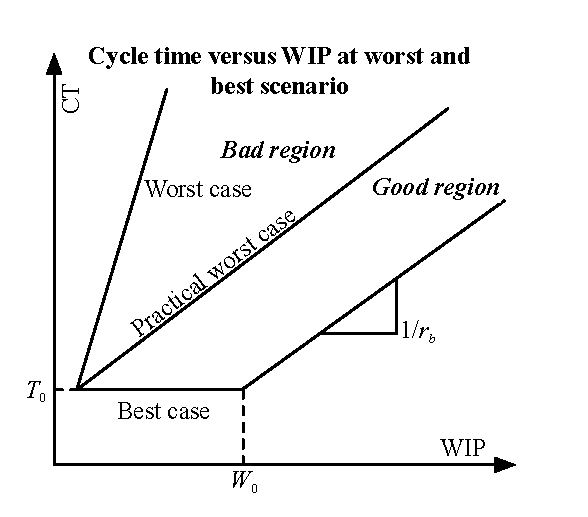
\includegraphics[width=.5\linewidth]{Figures/LiteratureReview/Cycle_time_versus_WIP}
  \caption{Cycle time versus WIP}\label{fig:Cycle time versus WIP}
  \source{Adapted from \citet*[p. 234]{Hopp2001}}
\end{figure}

\begin{figure}[H]
  \centering
  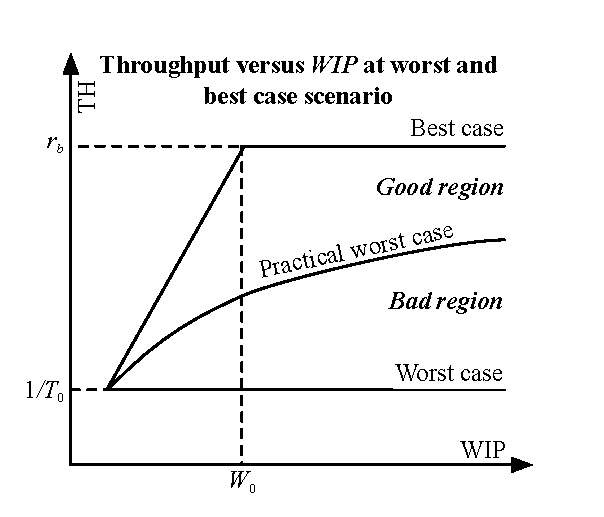
\includegraphics[width=.5\linewidth]{Figures/LiteratureReview/Throughput_versus_WIP}
  \caption{Throughput versus WIP worst- and best-case performance scenario}\label{fig:throughput versus WIP worst- and best-case performance scenario}
  \source{Adapted from \citet*[p. 234]{Hopp2001}}
\end{figure}

\subsubsection{Law (variability)}
\label{sec:org08dcdac}

The impact of variability in manufacturing systems is straightforward, increasing variability always degrades the performance of a production system \citep{Hopp2001}.
Because of the damages that variability can cause in a production system, several strategies aim at protecting the system from variability.

\subsubsection{Law (variability buffering)}
\label{sec:org8394cbe}

The most common are the use of buffers as a bumper or cushion.
The buffering method is the excess of at least one of the variables that can be consumed without harming the system's performance.
Variability in a production system will be buffered by some combination of inventory, capacity and time \citep{Hopp2001}.
In circumstances where buffers are ineffective, variability may propagate through transformation process impacting the production flow.
Thus, laws concerning the production flow, material flow, capacity, utilization, and variability propagation must be enunciated.

\subsubsection{Law (conservation of material)}
\label{sec:org7283fab}

The first law regarding the production flow is the conservation of material in and out of the transformation processes \citep{Hopp2001}.
Law (Conservation of Material) states that in a stable system, over the long run, the rate out of a system will equal the rate in, less any yield loss, plus any parts production within the system.
It means that in a system at steady state the flow of material is constant, consuming the necessary and only the necessary material to produce the goods.
It includes the ordinary transformation rate and loss of material.

\subsection{Law (capacity)}
The concept of stability in manufacturing systems requires that the input rate in transformation processes must be less than capacity, \(\mbox{THs}_{\mbox{max}}\).
The reason again is variability.
If the input rate equals capacity, any variation in the transformation processes may degrade the process performance.
The difference between the input rate and capacity creates a buffer that should grant the system stability by absorbing any minor variability.
In steady state, all plants will release work at an average rate that is strictly less than the average capacity \citep[p.303]{Hopp2001}.

\subsubsection{Law (utilization)}
\label{sec:org6048df1}

Law (Utilization) states that if a station increases utilization without making any other changes, average WIP and cycle time, CT, will increase in a highly nonlinear fashion \citep[p.303]{Hopp2001}.
An increase in process utilization unaccompanied by adjustments means a larger actual output for a same maximum output.
In the production line, it is an increase in bottleneck utilization, once the \(\mbox{THs} = \mbox{`bottleneck utilization'}\times\mbox{`bottleneck rate'}\).
Hence, according to Little's law for operation management (Equation\textasciitilde{}\ref{eq:Little's Law for operation management}) produces a nonlinear effect in WIP and CT.

\subsubsection{Law (process batching)}
\label{sec:org821fc3d}

Finally, the Law (Process Batching), accounts for finite production, i.e., in batch production where there are meaningful setup times.
According to Hopp and Spearman \cite{Hopp2001}, in batch production:

\begin{itemize}
    \item the minimum process batch size that yields a stable system may be greater than one;
    \item as process batch size becomes large; cycle time grows proportionally with batch size, and;
    \item cycle time at the station will be minimized for some process batch size, which may be greater than one \citep[p.306]{Hopp2001}.
\end{itemize}

The Figure\textasciitilde{}\ref{fig:Cycle time versus parallel batch size in batch production} illustrates these general relations between the batch size and the average cycle time.

\begin{figure}[H]
  \centering
  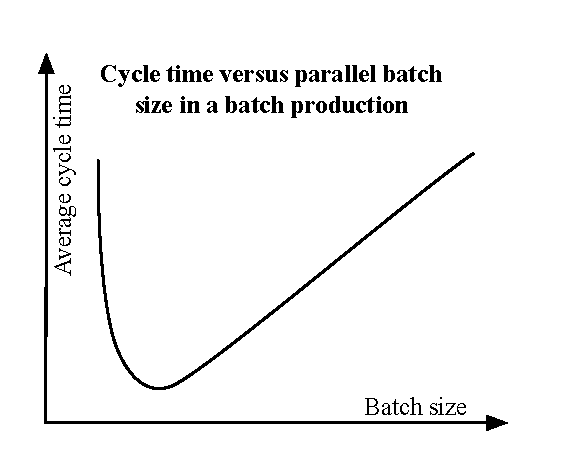
\includegraphics{Figures/LiteratureReview/Cycle_time_versus_parallel_batch_size_in_a_batch_production}
  \caption{Cycle time versus parallel batch size in batch production}\label{fig:Cycle time versus parallel batch size in batch production}
  \source{Adapted from \citet*[p.308]{Hopp2001}}
\end{figure}

The relationships between the concepts of lower level variables rely on stable production systems, where variability performs a minor role and does not disrupt the system.
Moreover, these relationships depend on a system running for a long period that can be considered infinite.
In batch production, where the process does not run continuously, the batches size are large enough producing a stable system.
However, not all system are stables, at steady state or with a minimum influence of external variability.
Transformation processes in shop job and one-of-a-kind manufacturing frequently do not exist for a long period.
Some processes exist only for a short period never making it to steady state.
To non-steady processes, a different approach must be used to.
The approach also may produce explanations of stable systems to point out algebraic relations between all system that could be used to analyze and prescribe management actions undertaken to improve the processes.

\subsection{The manufacturing theory does not apply directly to construction}
\label{sec:org960c3d7}

Manufacturing is either a continous or a repective process.
Machinery and human resources are specialized and qualified.
Production flow and material routes are established. 
Thus, most manufacturing processess can be automated.
That scenario is different from construction.
While capacity is knwon and measured in manufacturing, there was no way to measured it in construction.
Increasing production in construction often means add more human resources.
That often cause decrease of productivity due to lack of space, tools, skills, etc.

\section{Productivity Function [0/2]}
\label{sec:orgfb0ca8c}
\subsection{Production process system representation [100\%]}
\label{sec:org82c6769}

\begin{itemize}
\item[{$\square$}] A SYSTEM VIEW (Source: Identification of repetitive processes at steady- and unsteady-state: Transfer function)
Mathematical models have enabled a comprehensive understanding of production mechanisms supporting practices to improve production in manufacturing.
Hopp and Spearman (1996) committed to the comprehension of the manufacturing production system.
The system approach or system analysis was the problem-solving methodology of choice (\citep{Hopp2001}).
The first step of this methodology is a system view.
In the system view, the problem is observed as a system established by a set of subsystems that interact with each other.
Using the system approach, Hopp and Spearman elaborated significant laws to queue systems and the general production in manufacturing.
The conservation of material and capacity laws (Hopp and Spearman, 1996) are particularly attractive, not only according to their importance, but also because they explicitly state one or more system restrictions.

In this system view, an input is applied to a process to produce an output.
These three elements constitute a input/output system (Figure \ref{:fig_simple_system});  which we will refer simply as system from now on.
Input are, for instance, materials, tools, equipment, labor, management, time, and weather conditions \textbf{(Blanchard and Fabrycky, 2011)}.
\textbf{``Some of these factors, such as material, also become a part of the output product, while others are needed for control purposes (e.g., management) (\citep{Remold1989}).''}
The outputs are (usually) the product of the processes, for example, absolute quantities such as squared meters of plastered wall, meters drilled or relative measurement of progress such as the percentage of activity completion (\citep{Antunes2016}).
\uline{This last may be especially useful for Lean Construction practitioners that utilize the Planned Percent Complete (PPC) as the tracking tool.}
The process is the transformation procedure, or operation that when applied the input will create the output.
For instance, platerboads installation an drilling for the ouputs aforementioned.
The Figure \ref{:fig_simple_system} shows a single output and single input (SISO) for simplicty purposes.
A system can be composed by multiple inputs to single or multiple outputs (MISO and MIMO respectively) and also single input to multiple outputs.
Regardless of the system composition in terms of how many inputs and outputs or what the input(s), output(s) and process are; there are a few restrictions to a system:
\begin{itemize}
\item There is no output on lack of input.
\item There is no output without a process.
\end{itemize}
\end{itemize}


\begin{figure}[htbp]
\centering
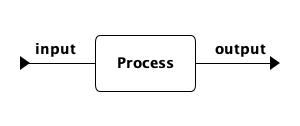
\includegraphics[height=150]{Figures/system_basic.png}
\caption{\label{fig:org533d345}Simple system}
\end{figure}


\begin{itemize}
\item[{$\square$}] Project as cycle
Most projects follow a cycle similar to plan-do-check-act (PDCA), also originally developed for manufacturing operations.
PDCA applies to continuous process improvement (Rumane and Badiru, 2013, p.53) and consists of a four-stages infinite loop.
First, the team establishing goals and develop the strategies to achieve them, creating a plan.
Second, the plan is then implemented.
The team carries out the actions addressing key points, according to the plan.
Third, the team measures the outcomes of their actions comparing the results to the goals.
Fourth, where the current process performance matches the goal, the team institutionalizes the new process’s performance, thus setting a benchmark, as well as the actions performed to achieve the goal, thus creating standard procedures.
In the case where the actions are not effective, the team must return to the first cycle stage.
The PDCA cycle restarts to implement further improvements.
\emph{In certain way, it means a system that is being constantly feedback by the current output state.}
\emph{If the current ouput state is no the one desired, the input will change to match achieve the output goal.}
\emph{The process improvement itself will alter the process as such the system will have increased the output using a constany input.}
/In terms of system, it will look like figure \ref{:closed_loop}.
The `plan' is desired ouput.
`Check' is a comparison between the `plan' and the current output.
The result is the measured `deviation'.
Based on the `deviation' actions must be implemented.
For example, the plan establish that an output of 50 square meters should be installed an hour to complete the job on time.
Two workers are initially assigned to the job (input).
If the two workers (input) are capable to install (process). 
That creates an action which for this example is to increase workers to increase output.
On the other hand, if the workers produce a higher output than the plan, the deviation will work on the other way: decrease the number of workers to reduce output thus matching the plan.
This configuration is a Closed-loop Control System or feedback control system in control theory.
\end{itemize}


\begin{center}
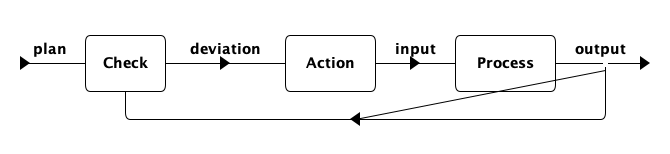
\includegraphics[width=.9\linewidth]{Figures/system_feedback_loop.png}
\end{center}

\# \#+ATTR\textsubscript{HTML}: :height 300

\begin{center}
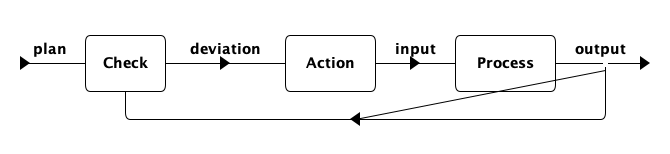
\includegraphics[width=.9\linewidth]{Figures/system_feedback_loop.png}
\end{center}






\begin{figure}[htbp]
\centering
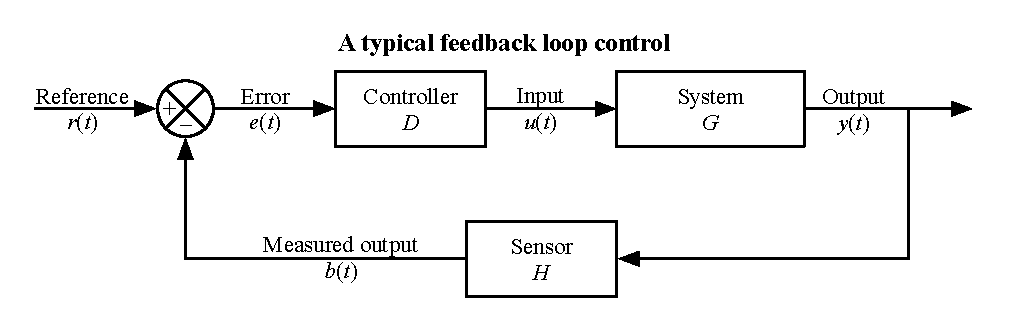
\includegraphics[height=150]{./Figures/A_typical_feedback_loop_control.eps}
\caption{\label{fig:orga63d77d}A typical feedback loop control}
\end{figure}


\begin{itemize}
\item[{$\square$}] Construction System
\uline{Source Paper07} Stays here

Several elements found in this literature review connect the characteristics of construction projects to the characteristics of a dynamic system.
As shown in Figure \ref{fig_construction_project-driven_production_system}, the interconnectivity is explicit between project stages, in the event that subsequent phases rely on the accomplishment and performance of previous ones.
This dependent connection remains valid for divided n-substages or n-activities and also applies to the proposed framework.
The dependence of processes and/or activities is well documented in the literature and well known by practitioners.
An activity or stage may impair or favour a successive action depending on the level of correlation and dependence.
The interdependence of activities forms a conduit to the propagation of unsure events. Potential risks captured through the entire project life may impact project execution whenever not properly treated, resulting in project deviations.
This sequence of events is represented in the system by the flow of uncertainty to risk and the occurrence of risk events, through risk management filtering actions—avoidance, acceptance, sharing, transference, mitigation, motivation—and, finally, to variability.
This flow resembles an intrinsic characteristic of systems in the presence of disturbance or noise.

Control systems may transmit unfiltered noise across connections affecting vulnerable components and causing disturbances or unpredicted behaviour.
Although the level of influence in this flow of sequential, parallel or overlapping relationships in the process or activity network have not been investigated at this point, understanding how risk transforms into variability, and especially how variability affects networked activities, propitiates an opportunity to develop methods aimed at avoiding and mitigating (filtering) the propagation of risk (noise). Regarding risk materialization in variability, different outcomes build on how concentrated or distributed the risk impact was.
Operating on possibly the same conditions of linear/nonlinear, deterministic/stochastic, time-domain/frequency domain, direct/inverse problems, discrete/continuous models---control theory may create a proxy theory to explain the effects of variability in construction projects by extending the elements of the dynamic systems.
\end{itemize}


\begin{figure}[htbp]
\centering
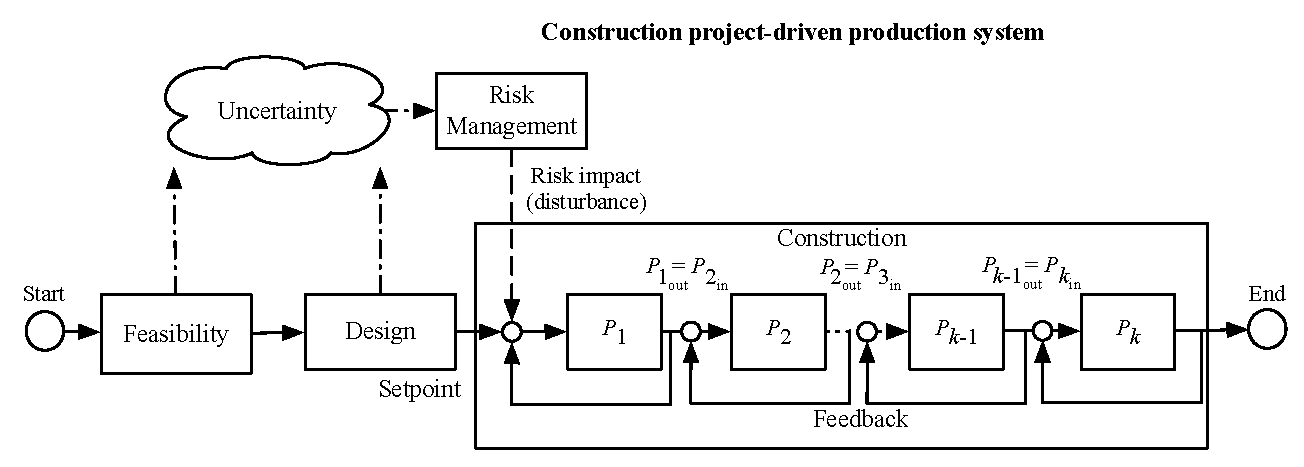
\includegraphics[height=150]{./Figures/Construction_project_driven_production_system.eps}
\caption{\label{fig:orgc9b4a7a}Construction project-driven production system}
\end{figure}


The simplest model of construction processes considers a closed conversion process where all factors affecting the work are steady state \citep{Drewin1982}.
In this model, the relationship between output and input, i.e., productivity, is given by a constant which is unaffected by external factors.
This constant can be determined by, for instance, the linear curve fitting or the ratio of the sum of outputs to the sum of inputs.
The linear scheduling method (LSM) (\citep{Harmelink1998,Su2016}) and line-of-balance (LOB) (\citep{Lumsden1968,Su2016,ZolfagharDolabi2014}) are examples of scheduling models for repetitive processes based on the steady state model.
However, ``because of the steady state nature of this model, the system more closely represents industrial production processes than construction processes (\citep{Thomas1990}).''
Short production runs \citep{Bashford2005}, high levels of output and input variability \cite{Gonzalez2009}, and nonlinear input-output relationships \citep{Bertelsen2003,Lutz1993} frequently prevent repetitive production processes in construction to reach steady state \citep{Antunes2015a,Walsh2007}.


\begin{itemize}
\item[{$\square$}] Limitations of Manufacturing system view to construction
These laws place reliance on stable systems, with long runs and at steady-state conditions.
However, production in project-based systems, such as construction, involves a mix of processes in steady- and unsteady-state, short and long production runs, and different learning curves (\citep{Antunes2015})
Hence, unless a construction process fulfills the stability and steady-state conditions, the manufacturing model and, consequently, the laws do not accurately represent production in construction.
Alternatively, variants of manufacturing laws must be developed to production in project-based systems that not fulfill those requirements.
\texttt{In this scenario of variety, it is crucial distinguishing between project-based systems conditions, comprehending process dynamics and its behavior.}
\end{itemize}


\subsection{Mathematical foundation of the Productivity Function}
\label{sec:orgd97c68c}

(Explain differential equations, the frequency domain and transformation)

Although much work has been done on production management of repetitive construction processes, more studies need to be conducted to develop equations to quantify project-driven production systems in construction.
The objective of this paper is to formulate variants of manufacturing production equations to calculate the production performance of repetitive construction processes for benchmarking purposes.
Furthermore, this paper shows the calculation of theoretical production parameters such as capacity and cycle time, as well as the influence of transient time on productivity.
The contribution of this paper to the body of knowledge are algebraic equations based on a generic model to calculate production parameters for repetitive processes in construction.

\subsubsection{Step response: Transient and steady state (explain the equation, move it, or clean it)}
\label{sec:org6bb2df8}

The transient is the immediate system reaction of an input change from a rest state \citep{Ogata2010}.
If the system is stable, the response will tend to a constant value, \(y_{\mbox{ssv}}\), when the time, \(t\), goes to infinity (Equation\textasciitilde{}\ref{eq:steady state}).
When the output reaches this value, the response is then at steady state.
The time that the system response takes from the moment the input changes to the steady state \citep{Nise2010,Ogata2010}, is the settling time, \(t_s\), i.e., the duration of the transient state.
Figure\textasciitilde{}\ref{fig_FIG02StepAnalysis} shows the step analysis which is an artificial and controlled way to reproduce the transient, as well as determine the steady state response of a system represented by the Productivity Function.
In the unitary-step function, \(u_{\mbox{step}}(t) \overset{\underset{\mathrm{\mathcal{L}}}{}}{\leftrightarrow} U_{\mbox{step}}(s) = 1/s\), at a time \(t_0\) the input changes from 0 to 1 and then is kept constant at 1.
At \(t_0\), if there is no delay, the system will notice the change in the input generating the transient response.
A physical interpretation of the step function is switching on a light by pressing a button.
Finally, if the system is stable; the output will tend to the steady state value.

\begin{equation}\label{eq:steady state}
	y_{\mbox{ssv}} = \lim_{t\rightarrow \infty} y(t)
\end{equation}

The step function in the time domain is given by:

\begin{equation}\label{eq:Step function in time domain P7}
	u_{\mbox{step}}(t) =
	\begin{cases}
 	0, & t = 0 \\
  	1, & t \ne 0
	\end{cases}.
\end{equation}

\subsubsection{TODO Explain transient and steady-state (move to section above, foundation)}
\label{sec:orgd69a76b}
\begin{itemize}
\item[{$\square$}] Why the transient
TRANSIENT STATE, STEADY-STATE, AND UNSTEADY-STATE RESPONSE
Two parts compose a system response in the time domain, transient, and steady- or unsteady-state.
Transient is the immediate system response to an input from an equilibrium state.
After the transient state, a system response can assume a steady- or unsteady-state.
In a stable system, the output tends to a constant value when \(t→∞\) (Mandal, 2006).
When the system response enters and stays in the threshold around the constant value the system reached the steady-state (Mandal, 2006).
The time the stable system takes to reach the steady-state is the settling time, \(t_s\).
On the other hand, if the response never reaches a final value or oscillates surpassing the threshold when \(t→∞\) the system is then at unsteady-state.
Consequently, the system outputs at unsteady-state vary with time during the on-time interval even induced by an invariable input.
\end{itemize}

\begin{enumerate}
\item Mathematical foundation of production (repeated title)
\label{sec:org0068401}

Repetitive construction projects falls into a fuzzy area where both project management and manufacturing overlap.
Repetitive construction projects are constituted by several contractors executing processes that they are specialized in, as for instance plumbers and electricians, that in the end, build a one-of-a-kind product.
The operations executed by several contractors are often performed repeatedly, and simultaneously at times, which stands for one of the peculiarities of repetitive projects.
In project-driven production, the coexistent mix of characteristics from project management and manufacturing makes the management of project-driven production problematic.
Project-driven production systems, such as repetitive construction, involve a combination of processes at transient, unsteady state, and-rarely-at steady state \citep{Antunes2015a,Antunes2015,Bashford2005,Walsh2007}.
However, traditional construction management, at this time, utilizes practices based on the manufacturing model that lacks the mathematical foundation to model and manage production in the project-driven systems \citep{Bertelsen2003,McCray2002,Pereira2013,Ko2016}.

\begin{itemize}
\item The system steady-state.
The steady-state of a system
\end{itemize}

\item Explain traditional methods of steady-state
\label{sec:org5999963}
The transient is the immediate system reaction of an input change from a rest state \citep{Ogata2010}.
If the system is stable, the response will tend to a constant value, \(y_{\mbox{ssv}}\), when the time, \(t\), goes to infinity (Equation\textasciitilde{}\ref{eq:steady state}).
When the output reaches this value, the response is then at steady state.
The time that the system response takes from the moment the input changes to the steady state \citep{Nise2010,Ogata2010}, is the settling time, \(t_s\), i.e., the duration of the transient state.
Figure\textasciitilde{}\ref{fig:Transient} shows the step analysis which is an artificial and controlled way to reproduce the transient, as well as determine the steady state response of a system represented by the Productivity Function.
In the unitary-step function, \(u_{\mbox{step}}(t) \overset{\underset{\mathrm{\mathcal{L}}}{}}{\leftrightarrow} U_{\mbox{step}}(s) = 1/s\), at a time \(t_0\) the input changes from 0 to 1 and then is kept constant at 1.
At \(t_0\), if there is no delay, the system will notice the change in the input generating the transient response.
A physical interpretation of the step function is switching on a light by pressing a button.
Finally, if the system is stable; the output will tend to the steady state value.

\begin{equation}\label{eq:steady state}
	y_{\mbox{ssv}} = \lim_{t\rightarrow \infty} y(t)
\end{equation}


\begin{figure}[htbp]
\centering
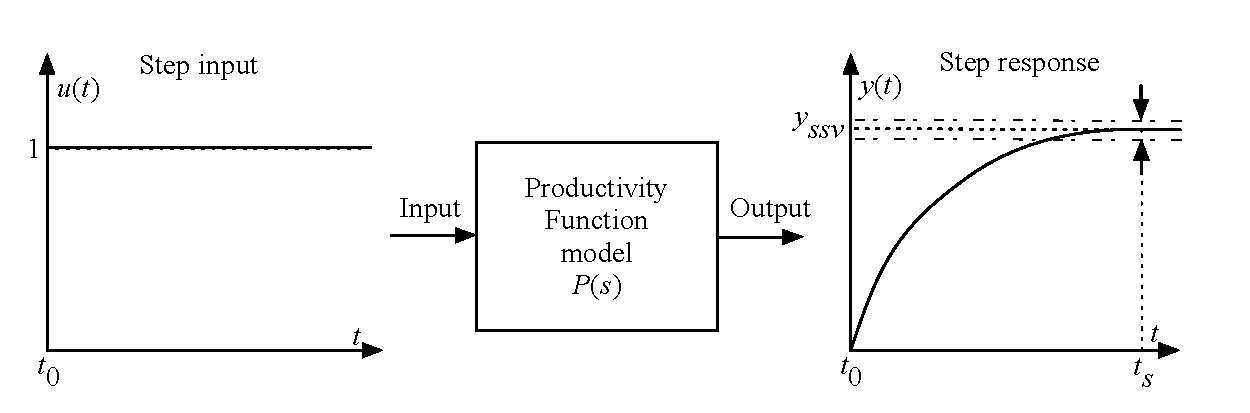
\includegraphics[height=150]{./Figures/FIG02Transient_analysis.eps}
\caption{\label{fig:orgf2f55a2}Transient analysis for unit step input \label{fig:Transient}}
\end{figure}


The step function in the time domain is given by:

\begin{equation}\label{eq:Step function in time domain P7}
	u_{\mbox{step}}(t) =
	\begin{cases}
 	0, & t = 0 \\
  1, & t \ne 0
	\end{cases}.
\end{equation}

The production of products or services designed to fulfill unique, or one-of-a-kind, specifications is the essence of project-driven production, also known as project-oriented manufacturing \citep{Martinez1997}.
``Repetitive construction projects are resource-driven, multi-unit projects characterized by activities which need to be performed in a sequence from unit to unit repeatedly \citep{Hajdasz2015}.'' That assumes a position in Product process matrix (Figure\textasciitilde{}\ref{fig:F01}) between manufacturing and project management, hence mixing characteristics from both sides, following the manufacturing production structure on the make-to-order (or make-to-build) demand of projects.
The product-process matrix (Figure\textasciitilde{}\ref{fig:F01}) illustrates the relationship of different products regarding their workflow and volume.
The most visible characteristic of the figure is a diagonal arrangement of the products showing a directly proportional relationship between production volume and workflow connection \citep{Kumar2009}, and also a relationship between the degree of freedom and production focus.

At the lower end of the diagonal, products are produced in high volume units and with hardly any or no differentiation at all, e.g., commodities.
Furthermore, the production process matches the characteristics of long run production \citep[p.154]{Baye2010} and economies of scale \citep[p.185]{Baye2010}.
The work stream is a continuous flow of specialized processes and equipment running at peak efficiency with stable and low variation processes \citep[pp.8-10]{Hopp2001} and relative short transients.


\begin{equation}\label{eq:Productivity_Function}
	P(s) = \frac{Y(s)}{U(s)} =
	\frac{(\beta_m s^m + \beta_{m-1} s^{m-1}+\ldots+\beta_0)}{(\alpha_n s^n + \alpha_{n-1} s^{n-1}+\ldots+\alpha_0)}
\end{equation}


\begin{itemize}
\item[{$\square$}] Transfer Function (Source: Identification of repetitive processes at steady- and unsteady-state: Transfer function)
\end{itemize}

The transfer function of a system, G, is a transformation from an input function into an output function, capable of describing an output (or multiple outputs) by an input (or multiple inputs) change, \(y(t) = G(t) \star u(t)\).
Although generic, the application of the transfer function concept is restricted to systems that are represented by ordinary differential equations (Mandal, 2006).
Ordinary differential equations can represent most dynamic systems in its entirety or at least in determined operational regions producing accurate results (Altmannand Macdonald, 2005; Mandal, 2006).
As a consequence, the transfer function modeling is extensively applied in the analysis and design of systems (Ogata, 2010). A generic transfer function makes possible representing the system dynamics by algebraic equations in the frequency domain, \(s\).
In the frequency domain, the convolution operation transforms into an algebraic multiplication in s, which is simpler to manipulate. Mathematically, “the transfer function of a linear system is defined as the ratio of the Laplace transform of the output, y(t), to the Laplace transform of the input, u(t), under the assumption that all initial conditions are zero” (Mandal, 2006), Equation 1.
Where the highest power of \(s\) in the denominator of the transfer function is equal to n, the system is called a nth-order system.
\end{enumerate}


\subsection{Modelling method [0/0]}
\label{sec:org340113a}

\begin{itemize}
\item[{$\square$}] SYSTEM IDENTIFICATION (Source: Identification of repetitive processes at steady- and unsteady-state: Transfer function)
(It should be moved after the system. To system Modelling approach.)
The objective of system identification is to build mathematical models of dynamic systems using measured data from a system (Ljung, 1998).
There are several system identification approaches to model different systems, for instance, transfer function.
The transfer function is particularly useful because it provides an algebraic description of a system as well means to calculate parameters of the system dynamics and stability.
Nevertheless, the modeling capability of the transfer function in construction must be evaluated and tested.
In this study, the modeling approach, i.e., transfer function, focuses on replicating the input/output “mapping” observed in a sample data. When the primary goal is the most accurate replication of data, regardless of the mathematical model structure, a black-box modeling approach is useful.
Additionally, black-box modeling supports a variety of models (Bapat, 2011; Billings, 2013), which have traditionally been practical for representing dynamic systems.
It means that at the end of the modeling, a mathematical description represents the actual process performance rather than a structure biased by assumptions and restrictions.
Black-box modeling is a trial-and-error method, where parameters of various models are estimated, and the output from those models is compared to the results with the opportunity for further refinement.
The resulting models vary in complexity depending on the flexibility needed to account for both the dynamics and any disturbance in the data.
The transfer function is used in order to show the system dynamics explicitly   

\uline{Source Paper04}
\end{itemize}

The objective of system identification is to build mathematical models of dynamic systems using measured data from a system \citep{Ljung1999}.
There are several system identification approaches to model a variety of systems; for instance, transfer function.
The transfer function is particularly useful because it provides an algebraic description of a system as well means to calculate parameters of the system dynamics and stability.
Nevertheless, the modeling capability of the transfer function in construction must be evaluated and tested.
In this study, the modeling approach, i.e., transfer function, focuses on replicating the input/output `mapping' observed in sample data.
When the primary goal is the most accurate replication of data, regardless of the mathematical model structure, a black-box modeling approach is useful.
Additionally, black-box modeling supports a variety of models \citep{Bapat2011, Billings2013}, which have traditionally been useful for representing dynamic systems.
At the end of the black-box modeling, a mathematical description represents the actual process performance rather than a structure biased by assumptions and restrictions.
Black-box modeling is a trial-and-error method, where parameters of various models are estimated, and the output from those models is compared to the results with the opportunity for further refinement.
The resulting models vary in complexity depending on the flexibility needed to account for both the dynamics and any disturbance in the data.
The transfer function is used to show the system dynamics explicitly.

\subsection{Production Theory for Construction}
\label{sec:orga27663c}
\subsubsection{Production forecast}
\label{sec:org074157e}

Forecasting is a tool that allows managers to create and access different scenarios of production result of risk impact.
Hence, forecasting supports both risk management practices for mitigating risk as the result of current progress on future completion.
Even though forecasting in construction is often inadequate and one of the weakest project controls functions \citep{ConstructionIndustryInstitute2012}.
``While there are many reasons for poor forecasting practice, one of the main causes may be the limited educational resources available on forecasting
In many textbooks and manuals, education about forecasting starts and stops with a presentation of earned value and elementary trending calculations \citep{ConstructionIndustryInstitute2012a},'' such as linear functions and averages.
The numerical estimation approach of Productivity Function can be embedded in the Project Management software or used as a stand-alone tool to forecast, access and simulate critical processes that require in-depth project controls.
As the Productivity Function models do not require anything else than the process' inputs and outputs, e.g., labor hours used to produce square meters of plastered wall, the models can be used together with project control practices such as earned value or Planned Percent Complete (PPC).
Simply by replacing the traditional steady state model by the Productivity Function, more accurate results should be obtained.
Furthermore, Dynamics Simulation, which relies on the mathematical models defined by ordinary differential equations (as the Productivity Function), have a significant role in supply chain \citep{Higuchi2004} and production in manufacturing \citep{Forrester1997}.
The application of Dynamics Simulation in construction is rare, specifically due to the lacking of mathematical models to describe the production in construction.
A gap that may be fulfilled by the Productivity Function.
While the algebraic form of Productivity Function may support the development of equations that further explain the production of project-driven processes, such as equations for capacity and cycle time.
Furthermore, the measurement and visualization of the transient state of project-driven processes support the quantitative and structured application of methods to reduce setup times, as for instance, Single Minute Exchange of Dices (SMED) and pre-fabrication \citep{Antunes2016}.

This chapter initiated as an exploration of elements in the building construction project cycle and their effect on production behavior, resulting in theoretical framework structured as a system \citep{Antunes2015a}.
This system proposed a flow of uncertainty to risk and then risk impact risk impact that would cause variability.
Following the framework, an analytical technique to describe the dynamic conditions of production in repetitive processes in projects was suggested \citep{Antunes2015}, as well as the relationship between the model characteristics and flow variability \citep{Antunes2016}.
This study is a step forward towards the development of a mathematically driven production theory for construction project management and project-driven systems defining a modeling approach and pointing out that dynamical systems theory would be useful to describe the behavior of production in construction.

\subsubsection{Variability analysis}
\label{sec:orgb052e05}
``Law (Variability): Increasing variability always degrades the performance of a production system \citep{Hopp2001}.''
In other words, the system will achieve its maximum performance when there is no variability.
That becomes evident when analyzing CV (Equation\textasciitilde{}\ref{eq:CV}): the greater the coefficient of variation, CV$\backslash$@; lower is the mean output, \(\bar{y}\), i.e., \(\bar{y} \sim \mbox{CV}^{-1}\).
Based on the knowledge of dynamic systems, the lowest level of variation in the output (indistinctly used in this paper as throughput once the outputs of dynamic systems are time dependent) happens when the system is at steady state \citep{Nise2010,Ogata2010}.
Productivity Function can be used to determine the theoretical output at steady state, and consequently the cycle time, using the stationary conditions as shown in Equation\textasciitilde{}\ref{eq:LongRun}.

The output at steady state of a system represented by a Productivity Function in the frequency domain can be calculated using the final value theorem.
``The final value theorem provides an easy-to-use technique for determining this value without having to first invert the Laplace transform to determine the time signal \citep[p.97]{Chen2007}.''
Equation\textasciitilde{}\ref{eq:FinalValue} shows the final value theorem which gives the steady state value, \(y_{\mbox{ssv}}\), in the frequency domain.

\begin{equation}\label{eq:FinalValue}
	\lim_{t\rightarrow \infty} y(t)=\lim_{s\rightarrow 0} sY(s)
\end{equation}

Replacing \(Y(s) = U_{\mbox{step}}(s) \times P(s)\), where \(U_{\mbox{step}}(s)\) is the step function, \(1/s\): \(Y(s) = 1/s \times P(s)\)

\begin{equation}\label{eq:FinalValue2}
	\lim_{t\rightarrow \infty} y(t)=\lim_{s \rightarrow 0} s \frac{1}{s} \times P(s)
\end{equation}

Replacing the left side of the Equation\textasciitilde{}\ref{eq:FinalValue2} by Equation\textasciitilde{}\ref{eq:steady state} the result is the output at steady state, i.e., the system's highest throughput with lowest variation: capacity.

\begin{equation}\label{eq:Capacity}
	y_{\mbox{ssv}} = \lim_{s \rightarrow 0} P(s) = P(0)
\end{equation}

\subsubsection{Production benchmark}
\label{sec:org069009d}
\subsubsection{Production plan, monitoring, and control}
\label{sec:org3fdcd03}
\begin{enumerate}
\item Throughput
\label{sec:org8662bd1}
Throughput is the output (non-defective) of a production process in a defined period \cite{Hopp2001}.
Construction scheduling accuracy strongly depends on being able to coordinate resources to determine the processes throughput \cite{Cho2011}.
When the relationship between resources and throughput can be established;
it is possible to determine the necessary resources to achieve the desired performance \cite{Cho2011}.
The production workflow in construction is segmented, i.e., job shop, where ``jobs arrive in different forms and require different tasks, and thus the equipment tends to be relatively general purpose \cite{Hayes1979},'' equipment has different productivity/availability \cite{Ok2006}, and the increased labor resource frequently causes site congestion \cite{Cho2011}.
There is an endless list of human factors that influence the labor output, such as the workers' experience, skill, and age \cite{El-Gohary2014}.

The open conversion model \cite{Kellogg1981} considers internal, external, and also unknown influences to productivity in a hierarchical arrangement.
Despite being generic and industry-comprehensive, at the operational level the complexity of inputs, such as the cost of labor, capital, energy, and materials; and output, e.g., dollars, makes the use of the open conversion model impractical \cite{Thomas1990}.
Explicitly incorporating all factors that influence productivity in a model is a challenging task.

``The relationship between inputs and outputs is very complex and, in many cases, includes some unknown combined effects \cite{Ok2006}.''
Simplifications and assumptions have to be made; however, the models are often over simplified.

\item Cycle-time
\label{sec:org4b5cf5d}

The accumulated throughput over time results in units of a service or product produced over time.
The time taken to produce one output is the cycle time.
In a continuous system, the function of the output produced is given by the integral of the output.
At steady state, where the throughput is constant, the unitary area below the curve is given by the throughput, \(y_{\mbox{ssv}}\), multiplied by the cycle time (Equation\textasciitilde{}\ref{eq:Capacity}).
In other words, the area results from the time when the last output was produced, \(t_{j-1}\), minus the time when the production of the current output unit finishes \(t_j\), where \(j\) is the denotation of an element and \(j \in N^+\).
Hence, \(\Delta t_j=t_j-t_{j-1}\) is the time taken to produce the \$j\$th-output, i.e., cycle time, \(\mbox{CT}_j\).
Therefore, Equation\textasciitilde{}\ref{eq:CycleTime} is equivalent to Equation\textasciitilde{}\ref{eq:CT}.
As \(y_{\mbox{ssv}}\) should determine the capacity of the system, the cycle time at steady state is the shortest production time of the system while stable, i.e., cycle time (best).

\begin{equation}\label{eq:CycleTime}
	y_{\mbox{ssv}} \times (t_j-t_{j-1}) = 1, \quad\mbox{ or }\quad \Delta t_j = 1/y_{\mbox{ssv}}
\end{equation}

Different to the steady state, the throughput of the production system varies while the system is in the transient.
The unitary area under the throughput curve can be calculated by a limited integral, with \(t_{j-1}\) and \(t_j\) as lower and higher limits, respectively (Equation\textasciitilde{}\ref{eq:ArtifactJ}).
As the throughput decreases, the cycle time increases.
Hence, the maximum cycle time of the production system, i.e., cycle time (worst) is found at start-up when the throughput at time \(t_0\) is null.

\begin{equation}\label{eq:ArtifactJ}
	\psi_j = \int_{t_{j-1}}^{t_j} y(t)dt
\end{equation}

Considering that the production system will increase its throughput over time as per its transient curve; the cycle time (worst) is the time taken to produce the first output (\(j=1\)) from a rest state: \(\Delta t_m = t_1-t_0\), or simply \(\Delta t_j = t_1\), once \(t_0 = 0\), is given by Equation\textasciitilde{}\ref{eq:Artifact1}.

\begin{equation}\label{eq:Artifact1}
	\psi_1 = \int_{0}^{t_1} y(t)dt
\end{equation}

Consequently, if the process increases its throughput as described by its transient curve, the longer it will take to reach the steady state and the smaller will be the area under the curve; hence, smaller its average output produced per time.
The average output per time can be calculated by the average function value given by Equation\textasciitilde{}\ref{eq:Artifact2}.

\begin{equation}\label{eq:Artifact2}
	\psi_{t_s} = \frac{1}{t_s} \int_{0}^{t_s} y(t)dt
\end{equation}

In other words, for processes with equal capacity, \(y_{\mbox{ssv}}\), the longer the transient time, \(t_{s}\), the longer is the average cycle time, \(\bar{\mbox{CT}}\).
Also, for processes with equal transient time the greater the capacity, the smaller is the average cycle.

\begin{equation}\label{eq:CycleTime}
y_{\mbox{ssv}} \times (t_j-t_{j-1}) = 1, \quad\mbox{ or }\quad \Delta t_j = 1/y_{\mbox{ssv}}
\end{equation}

\begin{enumerate}
\item Average cycle-time
\label{sec:org60bea77}
\item Worst cycle-time
\label{sec:orgdc7f6d4}
\item Best cycle-time
\label{sec:orgb483dba}
\end{enumerate}
\item Capacity
\label{sec:org3ab4e68}
``Law (Capacity): In steady state, all plants will release work at an average rate that is strictly less than the average capacity \citep[p.]{Hopp2001}.''
Furthermore, in most cases, releasing work into the system above the capacity causes the system to become unstable \citep{Hopp2001}.
According to these definitions, it would be correct to state that a process' capability is the highest throughput achievable without the process becoming unstable.
Thus, at capacity, the process operates with optimal productivity \citep{Kisi2017}.
``The theoretical maximum productivity that would be achieved under absolutely perfect conditions in all respects (perfect weather, highly motivated, and productive labor with perfect workmanship, optimal materials, optimal equipment, no interferences from other trades, no design errors, perfect understanding of design intend, etc \ldots) \citep[p.150]{Son2011}.''

However, the variation in the efficiency of workers and equipment, actual demand, and scheduling planning and control\textasciitilde{}\cite[p.54]{Kumar2009} may prevent processes from achieving the system design capacity.
Design capacity in a manufacturing system is engineered to full-scale operating conditions.
However, the system capacity is less than the design capacity, because the full-scale operating conditions are rarely met \citep{Kumar2009}.

The capacity of project-driven processes is not engineered but based on intuition \citep{McCray2002,ProjectManagementInstitute2011}.
Regardless of the equation used for productivity measurement \citep{Thomas1990}, determining the system capacity is crucial to settling a benchmark and elaborating what the level of productivity the actual performance should be compared to \citep{Abdel-Razek2007,Olomolaiye1998,Zhao2014}.



\begin{equation}\label{eq:Capacity}
	y_{\mbox{ssv}} = \lim_{s \rightarrow 0} P(s) = P(0)
\end{equation}
\end{enumerate}


\section{Applicability}
\label{sec:org6687405}
\subsection{Automation and technology}
\label{sec:orgcebb1ec}
\subsubsection{Supervisory control and data acquisition (SCADA)}
\label{sec:org4825063}
\subsubsection{Challenges}
\label{sec:orgfbbb417}
\subsection{Decision-making support}
\label{sec:orgf9d302e}
\subsection{Benefits and impacts}
\label{sec:org33ace1f}
\section{Discussion}
\label{sec:org2715cf2}
\section{Conclusion}
\label{sec:orge46272c}

\section{Plan}
\label{sec:orgcaa325b}
\begin{center}
\begin{tabular}{lrlrr}
Section & Words & Current & Effort & Current\\
\hline
Plan &  &  & 1 & 1\\
Introduction & 500 &  & 4 & \\
Lean principles and production theory & 1500 &  & 5 & \\
Productivity Function & 2000 &  & 5 & 5\\
Applicability & 1500 &  & 5 & \\
Discussion & 1000 &  & 5 & \\
Conclusion & 500 &  & 5 & \\
Review &  &  & 5 & \\
\hline
Total & 7000 & 0 & 35 & 3\\
\end{tabular}
\end{center}
\subsection{6 Section}
\label{sec:orgad51ce3}

\section{References}
\label{sec:orgfd500f6}

\printbibliography[title=none]
\end{document}